% Preamble
\documentclass[11pt]{article}

% Packages
\usepackage{amsmath}
\usepackage{mathtools}
\usepackage{ragged2e}
\usepackage [utf8]{inputenc}
\usepackage{blindtext}
\usepackage{wrapfig}
\usepackage{xcolor}
\usepackage {polski}
\usepackage{multicol}
\usepackage[a4paper, total={5.7in, 8in}]{geometry}
\usepackage{graphicx}
\usepackage{amstex}
\usepackage{csvsimple}
\usepackage{changepage}
\usepackage{enumitem}
\usepackage[english]{babel}
\usepackage{biblatex}
\usepackage{caption}
\usepackage{indentfirst}
\usepackage{epstopdf-base}
\usepackage{textcomp}

% Document
\begin{document}
%    Nagłówek
    \begin{flushleft}
        Maciej Pierzchała 282 934 \hfill Data wykonania ćwiczenia:\\
        Filip Kubecki 272 655 \hfill 15 października 2024r\\
        \hfill Data sporządzenia sprawozdania:\\
        Grupa: Wtorek 10:35 \hfill 22 października 2024r\\
    \end{flushleft}

    \begin{center}
        \Large\textbf{Laboratorium 3}\\
        \textbf{Charakteryzacja czujników naprężenia}
    \end{center}
    \hfill
%    Treść
    \section{Spis przyrządów}
    \par{
        Do wykonania ćwiczenia wykorzystano:
        \begin{itemize}
            \setlength\itemsep{0em}
            \item[-] Piezoelektryczny czujnik naprężenia
            \item[-] Multimetr cyfrowy Sigilent SDM 3055
            \item[-] Suwmiarkę
            \item[-] Śrubę mikrometryczną
            \item[-] Przyrząd do kontrolowanego naprężania próbki
        \end{itemize}
    }
    \section{Przebieg i cele doświadczenia}
    \par Doświadczenie polegało na wyginaniu próbki piezorezystora grubowarstwowego wykonanego metodą sitodruku na podłożu z ceramiki
    alundowej przy pomocy śruby mikrometrycznej. Śruba pozwalała na precyzyjne ustalanie wartości wygięcia próbki (Interwał co 0.05 mm).
    Podczas wyginania próbki mierzono rezystancję w kierunku podłużnym oraz poprzecznym. Wartości mierzono podczas poddawaniu próbki stresowi
    oraz podczas relaksacji próbki. Pozwoli to wykreślić wykres histerezy oraz oreślić błąd nieliniowości oraz błąd histerezy.
    \section{Obliczenia i analiza wyników}
    \par Aby wykreślić wykres $\Delta R/R_0=f(\varepsilon)$ najpierw należy wyznaczyć wartość odkształcenia
    względnego ($\varepsilon$) dla każdego pomiaru.\\
    \indent Wartość odkształcenia względnego wyznaczono ze wzoru:
    \begin{gather*}
        \varepsilon=1.5\cdot\frac{t(L-x)}{L^3}\cdot f
    \end{gather*}
    \indent Gdzie:
        {\footnotesize
    \begin{itemize}
        \setlength\itemsep{0em}
        \item[] \textbf{$\varepsilon$} - odkształcenie względne próbki [m],
        \item[] \textbf{$t$} - grubość płytki [m],
        \item[] \textbf{$L$} - odległość między górną powierzchnią statywu a punktem ugięcia próbki [m],
        \item[] \textbf{$x$} - odległość między górną powierzchnią statywu a środkiem uginanego rezystora [m],
        \item[] \textbf{$f$} - ugięcie próbki [m],
    \end{itemize}}
    Podstawiając wartości z wykluczeniem $f$ gdyż jest ona zmienna, uzyskamy:
    \begin{gather*}
        \varepsilon=1.5\cdot\frac{0.00065[m](0.0322[m]-0.0011[m])}{(0.0322[m])^3}\cdot f =\\
        = 1.5\cdot\frac{0.00065[m](0.0311[m])}{0.000033386[m^3]}\cdot f = \\
        = 0.9082332342\dots [m^{-1}]\cdot f
    \end{gather*}
    Przykładowo dla wychylenia $x = 0.05 [mm]$:
    \begin{gather*}
        \varepsilon=0.9082332342\dots [m]\cdot 0.05 [mm] = \\
        = 0.9082332342\dots [m^{-1}]\cdot 5\cdot 10^{-5}[m] = 4.541166171\cdot 10^{-5}
    \end{gather*}
    \indent Wyliczanie wartości $\Delta R/R_0$ jest trywialne więc pominięto tłumaczenie tej kalkulacji.\\
    \indent Przy pomocy powyższych kalkulacji wyznaczono charakterystyki $\Delta R/R_0=f(\varepsilon)$ dla efektu podłużnego i poprzecznego (wykres 1 i 2):\\
    \noindent\makebox[\textwidth]{
        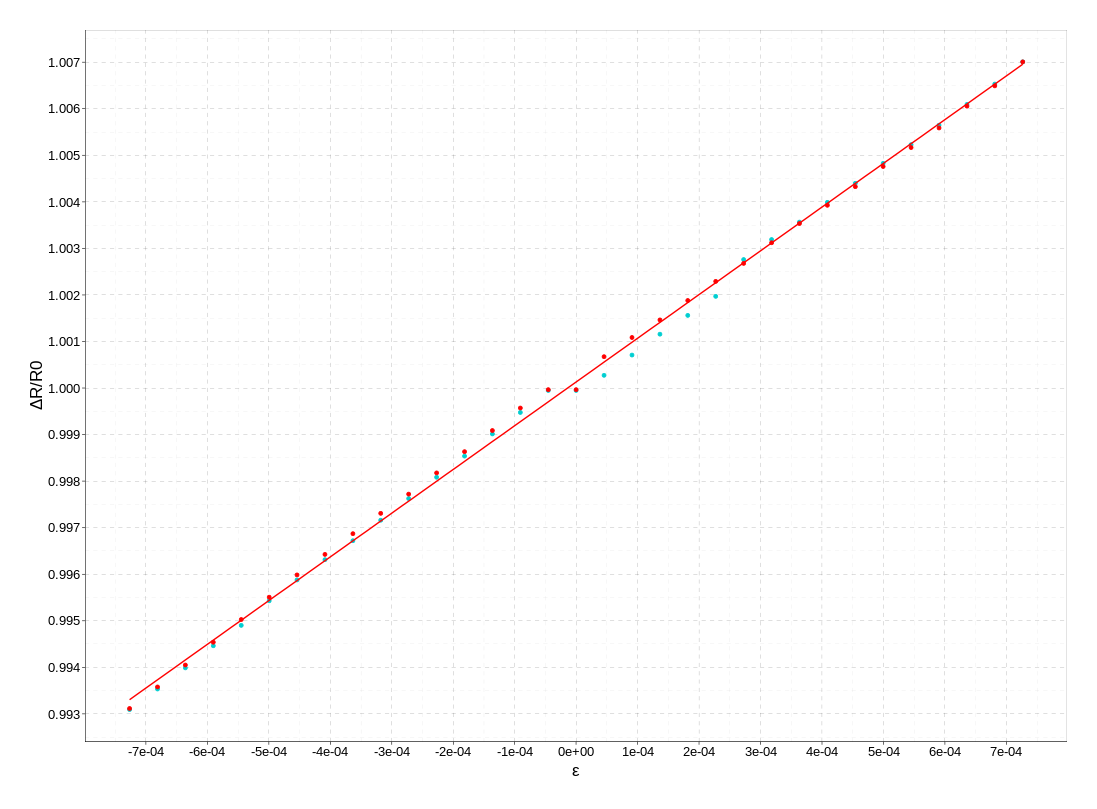
\includegraphics[scale = 0.4]{/home/bork/IdeaProjects/LatexProjects/src/PodstawyTechnikiSensorowej/Lab3/Img/podluzny.png}
    }
    \noindent\makebox[\textwidth]{
        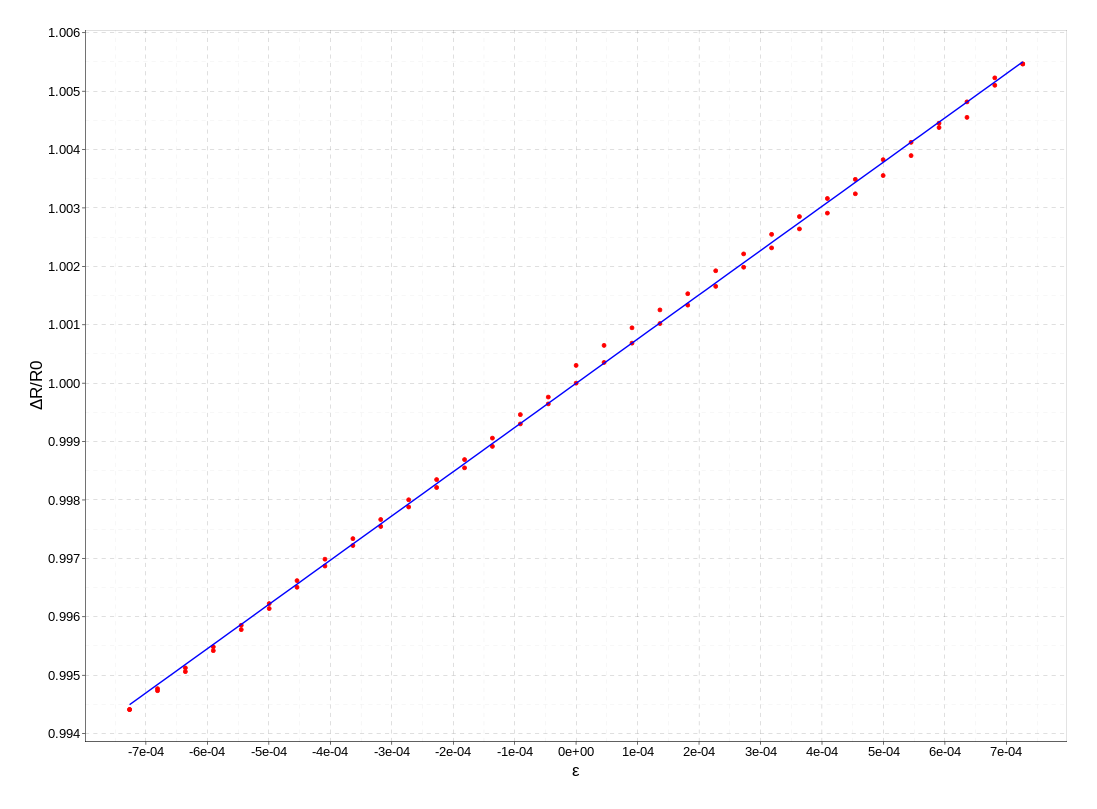
\includegraphics[scale = 0.45]{/home/bork/IdeaProjects/LatexProjects/src/PodstawyTechnikiSensorowej/Lab3/Img/poprzeczny.png}
    }
    \indent Na podstawie powyższych wykresów jesteśmy w stanie zaobserwować niewielką histerezę pomiaru. Wykreślono również
    aproksymację liniową wykonaną metodą regresji liniowej dla obu charakterystyk. \\

    \indent Poniżej zaprezentowano aproksymacje liniowe obu charakterystyk
    na jednym wykresie wraz z ich współczynnikami GF (czerwona linia - efekt podłużny, niebieska linia - efekt poprzeczny):\\
    \noindent\makebox[\textwidth]{
        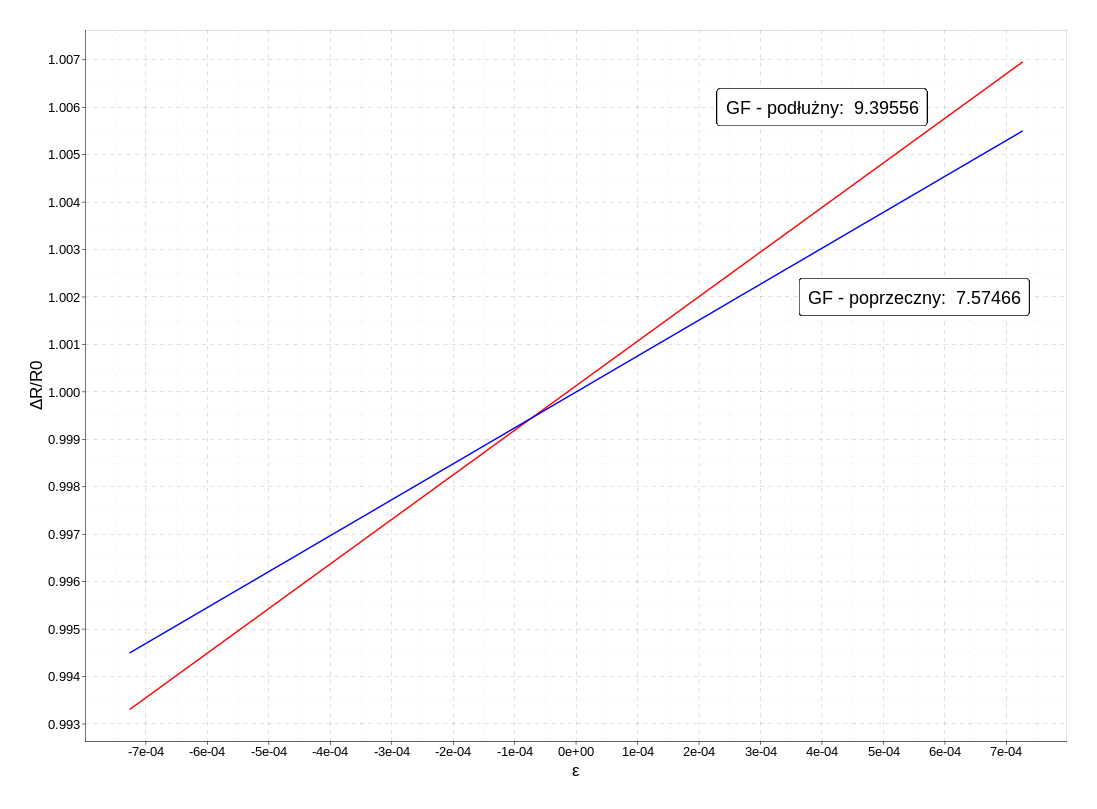
\includegraphics[scale = 0.45]{/home/bork/IdeaProjects/LatexProjects/src/PodstawyTechnikiSensorowej/Lab3/Img/both.png}
    }
    \indent Przy pomocy powyższych wykresów wyznaczono wartość błędu nieliniowości. Wykorzystano poniższy wzór:
    \begin{gather*}
        N=\frac{\Delta Y}{Y_{max}-Y_{min}}\cdot 100\%
    \end{gather*}
    \indent Gdzie:
        {\footnotesize
    \begin{itemize}
        \setlength\itemsep{0em}
        \item[] \textbf{$\Delta Y$} - wartość maksymalna wartości bezwzględnych różnic pomiędzy wartością wyznaczoną na podstawie równania prostej i wyników pomiarów,
        \item[] \textbf{$Y_{max}$} - wartość maksymalna,
        \item[] \textbf{$Y_{min}$} - wartość minimalna,
    \end{itemize}}
    \indent Wartość $\Delta Y$ wyznaczono oddzielno dla wykresu efektu poprzecznego oraz podłużnego. Dla obu
    charakterysyk wartość ta znajdowała się w punkcie $\varepsilon \approx 0.045$. Dla efektu podłużnego występowała ona
    dla wywierania stresu na próbkę a dla efektu poprzecznego podczas odpuszczania nacisku z próbki.
    \newpage
    \indent Ostatecznie wartość wyliczamyz poniższego równania wykorzystując wcześniej wyznaczone współczynniki kierunkowe:
    \begin{gather*}
        \Delta Y=(GF\cdot \varepsilon) - Y
    \end{gather*}
    Gdzie:
        {\footnotesize
    \begin{itemize}
        \setlength\itemsep{0em}
        \item[] \textbf{$Y$} - najmocniej odbiegająca wartość zmierzona,
        \item[] \textbf{$(GF\cdot\varepsilon)$} - wartość wynikająca z regresji liniowej,
    \end{itemize}}
    Przykładowo dla efektu poprzecznego:
    \begin{gather*}
        \Delta Y=(0.007574665\cdot 0.04541166)\cdot 1.0003549 = \\
        = 3.442\cdot 10^{-4}
    \end{gather*}
    Dla efektu poprzecznego:
    \begin{gather*}
        \Delta Y=4.126\cdot 10^{-4}
    \end{gather*}
    Teraz można wyliczyć błąd nieliniowości dla efektu podłużnego:
    \begin{gather*}
        N=\frac{4.126\cdot 10^{-4}}{1.007061-0.9931437}\cdot 100\% = \\
        = 0.029644 \%
    \end{gather*}
    Dla efektu poprzecznego:
    \begin{gather*}
        N=0.031136 \%
    \end{gather*}
    \\
    Ostatecznie należy wyliczyć jeszcze wartość błędu histerezy. Wyliczamy go z poniższego wzoru:
    \begin{gather*}
        H=\frac{max|Y_1-Y_2|}{Y_{max}-Y_{min}}\cdot 100\%
    \end{gather*}
    Przykładowo dla efektu podłużnego w punkcie $\varepsilon \approx 0.045$:
    \begin{gather*}
        H=\frac{max|1.0007260-1.000325|}{0.0139173}\cdot 100\%=\\
        = 0.028813 \%
    \end{gather*}
    Dla efektu poprzecznego:
    \begin{gather*}
        H=0.026396 \%
    \end{gather*}


    \section{Wnioski}
    \par Na podstawie wykonanych obliczeń oraz wykreślonych charakterystyk jesteśmy w stanie zaobserwować
    przewidywane zachowanie dla efektu podłużnego oraz poprzecznego w czujniku tensometrycznym. Współczynnik kierunkowy
    funkcji liniowej aproksymującej wykres charakterystyki dla efektu podłużnego jest większy niż dla efektu poprzecznego
    co wynikało z znanej nam teori mówiącej że efekt podłużny jest o wiele bardziej znaczący niż efekt podłużny.\\
    \indent Na wykresie ciężko zaobserwować charakterystyczny wykres histerezy. Wartości są porozsówane losowo prawdopodobnie z
    powodu wszystkich niepewności które występowały w procesie pomiaru: niepewność ustawiania wartości eksperymentatora, niepewność tensometru czy
    niepewność multimetru.



    %Bibliografia
    \vfill
    \footnotesize
    \begin{thebibliography}{3}
        \bibitem{texbook1}
        https://en.wikipedia.org/wiki/Piezoresistive\_effect
        \bibitem{texbook2}
        https://en.wikipedia.org/wiki/Strain\_gauge
        \bibitem{texbook3}
        https://www.microsensorcorp.com/Details\_what-is-pressure-hysteresis.html
    \end{thebibliography}
\end{document}